\documentclass[ twoside,openright,titlepage,numbers=noenddot,headinclude,%1headlines,% letterpaper a4paper
                footinclude=true,cleardoublepage=empty,abstractoff, % <--- obsolete, remove (todo)
                BCOR=5mm,paper=a4,fontsize=11pt,%11pt,a4paper,%
                ngerman,american,%
                ]{scrreprt}


%load fonts und useful packages. etc.
% ****************************************************************************************************
% classicthesis-config.tex 
% formerly known as loadpackages.sty, classicthesis-ldpkg.sty, and classicthesis-preamble.sty 
% Use it at the beginning of your ClassicThesis.tex, or as a LaTeX Preamble 
% in your ClassicThesis.{tex,lyx} with \input{classicthesis-config}
% ****************************************************************************************************  
% If you like the classicthesis, then I would appreciate a postcard. 
% My address can be found in the file ClassicThesis.pdf. A collection 
% of the postcards I received so far is available online at 
% http://postcards.miede.de
% ****************************************************************************************************

% ****************************************************************************************************
% 1. Configure classicthesis for your needs here, e.g., remove "drafting" below 
% in order to deactivate the time-stamp on the pages
% ****************************************************************************************************
\PassOptionsToPackage{eulerchapternumbers,listings,drafting,%
				 pdfspacing,%floatperchapter,%linedheaders,%
				 subfig,beramono,eulermath}{classicthesis}										
% ********************************************************************
% Available options for classicthesis.sty 
% (see ClassicThesis.pdf for more information):
% drafting
% parts nochapters linedheaders
% eulerchapternumbers beramono eulermath pdfspacing minionprospacing
% tocaligned dottedtoc manychapters
% listings floatperchapter subfig
% ********************************************************************

% ********************************************************************
% Triggers for this config
% ******************************************************************** 
\usepackage{ifthen}
\newboolean{enable-backrefs} % enable backrefs in the bibliography
\setboolean{enable-backrefs}{false} % true false
% ****************************************************************************************************


% ****************************************************************************************************
% 2. Personal data and user ad-hoc commands
% ****************************************************************************************************
\newcommand{\myTitle}{NUMERICAL SIMULATION OF PARTIAL DIFFERENTIAL
EQUATIONS\xspace}
\newcommand{\mySubtitle}{ Project Report\xspace}
\newcommand{\myDegree}{\xspace}
\newcommand{\myName}{Vincent Peeters and Moritz Wolter\xspace}
\newcommand{\myProf}{Stefan Vandewalle \xspace}
\newcommand{\myOtherProf}{Stefaan Poedts \xspace}
\newcommand{\mySupervisor}{\xspace}
\newcommand{\myFaculty}{\xspace}
\newcommand{\myDepartment}{\xspace}
\newcommand{\myUni}{KU Leuven\xspace}
\newcommand{\myLocation}{Leuven\xspace}
\newcommand{\myTime}{	\selectlanguage{american}
			\today \xspace}
\newcommand{\myVersion}{Version 1\xspace}

% ********************************************************************
% Setup, finetuning, and useful commands
% ********************************************************************
\newcounter{dummy} % necessary for correct hyperlinks (to index, bib, etc.)
\newlength{\abcd} % for ab..z string length calculation
\providecommand{\mLyX}{L\kern-.1667em\lower.25em\hbox{Y}\kern-.125emX\@}
\newcommand{\ie}{i.\,e.}
\newcommand{\Ie}{I.\,e.}
\newcommand{\eg}{e.\,g.}
\newcommand{\Eg}{E.\,g.} 
% ****************************************************************************************************


% ****************************************************************************************************
% 3. Loading some handy packages
% ****************************************************************************************************
% ******************************************************************** 
% Packages with options that might require adjustments
% ******************************************************************** 
\PassOptionsToPackage{utf8}{inputenc}	% latin9 (ISO-8859-9) = latin1+"Euro sign"
 \usepackage{inputenc}				

\PassOptionsToPackage{english}{babel}   % change this to your language(s)
% Spanish languages need extra options in order to work with this template
%\PassOptionsToPackage{spanish,es-lcroman}{babel}
 \usepackage{babel}					

 %\PassOptionsToPackage{square,numbers}{natbib}
 %\usepackage{natbib}
 \usepackage[fixlanguage]{babelbib}
 \selectbiblanguage{german}
 \bibliographystyle{babplain}

\PassOptionsToPackage{fleqn}{amsmath}		% math environments and more by the AMS 
 \usepackage{amsmath}

%When using tikZ one must also use the color package.
\PassOptionsToPackage{usenames,dvipsnames}{color}
 \usepackage{color}

%This package lets you compile tikz graphics.
 \usepackage{tikz}
 \usepackage{pgfplots}
 \usetikzlibrary{decorations.markings}
 \usepackage{standalone}

% ******************************************************************** 
% General useful packages
% ******************************************************************** 
\PassOptionsToPackage{T1}{fontenc} % T2A for cyrillics
	\usepackage{fontenc}     
\usepackage{textcomp} % fix warning with missing font shapes
\usepackage{scrhack} % fix warnings when using KOMA with listings package          
\usepackage{xspace} % to get the spacing after macros right  
\usepackage{mparhack} % get marginpar right
\usepackage{fixltx2e} % fixes some LaTeX stuff 
\PassOptionsToPackage{printonlyused,smaller}{acronym}
	\usepackage{acronym} % nice macros for handling all acronyms in the thesis
%\renewcommand*{\acsfont}[1]{\textssc{#1}} % for MinionPro
\renewcommand{\bflabel}[1]{{#1}\hfill} % fix the list of acronyms
% ****************************************************************************************************


% ****************************************************************************************************
% 4. Setup floats: tables, (sub)figures, and captions
% ****************************************************************************************************
\usepackage{tabularx} % better tables
	\setlength{\extrarowheight}{3pt} % increase table row height
\newcommand{\tableheadline}[1]{\multicolumn{1}{c}{\spacedlowsmallcaps{#1}}}
\newcommand{\myfloatalign}{\centering} % to be used with each float for alignment
\usepackage{caption}
\captionsetup{format=hang,font=small}
\usepackage{subfig}  
% ****************************************************************************************************


% ****************************************************************************************************
% 5. Setup code listings
% ****************************************************************************************************
\usepackage{listings} 
%\lstset{emph={trueIndex,root},emphstyle=\color{BlueViolet}}%\underbar} % for special keywords
\lstset{language=[LaTeX]Tex,%C++,
    keywordstyle=\color{RoyalBlue},%\bfseries,
    basicstyle=\small\ttfamily,
    %identifierstyle=\color{NavyBlue},
    commentstyle=\color{Green}\ttfamily,
    stringstyle=\rmfamily,
    numbers=none,%left,%
    numberstyle=\scriptsize,%\tiny
    stepnumber=5,
    numbersep=8pt,
    showstringspaces=false,
    breaklines=true,
    frameround=ftff,
    frame=single,
    belowcaptionskip=.75\baselineskip
    %frame=L
} 
% ****************************************************************************************************    		   


% ****************************************************************************************************
% 6. PDFLaTeX, hyperreferences and citation backreferences
% ****************************************************************************************************
% ********************************************************************
% Using PDFLaTeX
% ********************************************************************
\PassOptionsToPackage{pdftex,hyperfootnotes=false,pdfpagelabels}{hyperref}
	\usepackage{hyperref}  % backref linktocpage pagebackref
\pdfcompresslevel=9
\pdfadjustspacing=1 
\PassOptionsToPackage{pdftex}{graphicx}
	\usepackage{graphicx} 

% ********************************************************************
% Setup the style of the backrefs from the bibliography
% (translate the options to any language you use)
% ********************************************************************
\newcommand{\backrefnotcitedstring}{\relax}%(Not cited.)
\newcommand{\backrefcitedsinglestring}[1]{(Cited on page~#1.)}
\newcommand{\backrefcitedmultistring}[1]{(Cited on pages~#1.)}
\ifthenelse{\boolean{enable-backrefs}}%
{%
		\PassOptionsToPackage{hyperpageref}{backref}
		\usepackage{backref} % to be loaded after hyperref package 
		   \renewcommand{\backreftwosep}{ and~} % separate 2 pages
		   \renewcommand{\backreflastsep}{, and~} % separate last of longer list
		   \renewcommand*{\backref}[1]{}  % disable standard
		   \renewcommand*{\backrefalt}[4]{% detailed backref
		      \ifcase #1 %
		         \backrefnotcitedstring%
		      \or%
		         \backrefcitedsinglestring{#2}%
		      \else%
		         \backrefcitedmultistring{#2}%
		      \fi}%
}{\relax}    

% ********************************************************************
% Hyperreferences
% ********************************************************************
\hypersetup{%
    %draft,	% = no hyperlinking at all (useful in b/w printouts)
    colorlinks=true, linktocpage=true, pdfstartpage=3, pdfstartview=FitV,%
    % uncomment the following line if you want to have black links (e.g., for printing)
    %colorlinks=false, linktocpage=false, pdfborder={0 0 0}, pdfstartpage=3, pdfstartview=FitV,% 
    breaklinks=true, pdfpagemode=UseNone, pageanchor=true, pdfpagemode=UseOutlines,%
    plainpages=false, bookmarksnumbered, bookmarksopen=true, bookmarksopenlevel=1,%
    hypertexnames=true, pdfhighlight=/O,%nesting=true,%frenchlinks,%
    urlcolor=webbrown, linkcolor=RoyalBlue, citecolor=webgreen, %pagecolor=RoyalBlue,%
    %urlcolor=Black, linkcolor=Black, citecolor=Black, %pagecolor=Black,%
    pdftitle={\myTitle},%
    pdfauthor={\textcopyright\ \myName, \myUni, \myFaculty},%
    pdfsubject={},%
    pdfkeywords={},%
    pdfcreator={pdfLaTeX},%
    pdfproducer={LaTeX with hyperref and classicthesis}%
}   

% ********************************************************************
% Setup autoreferences
% ********************************************************************
% There are some issues regarding autorefnames
% http://www.ureader.de/msg/136221647.aspx
% http://www.tex.ac.uk/cgi-bin/texfaq2html?label=latexwords
% you have to redefine the makros for the 
% language you use, e.g., american, ngerman
% (as chosen when loading babel/AtBeginDocument)
% ********************************************************************
\makeatletter
\@ifpackageloaded{babel}%
    {%
       \addto\extrasamerican{%
					\renewcommand*{\figureautorefname}{Figure}%
					\renewcommand*{\tableautorefname}{Table}%
					\renewcommand*{\partautorefname}{Part}%
					\renewcommand*{\chapterautorefname}{Chapter}%
					\renewcommand*{\sectionautorefname}{Section}%
					\renewcommand*{\subsectionautorefname}{Section}%
					\renewcommand*{\subsubsectionautorefname}{Section}% 	
				}%
       \addto\extrasngerman{% 
					\renewcommand*{\paragraphautorefname}{Absatz}%
					\renewcommand*{\subparagraphautorefname}{Unterabsatz}%
					\renewcommand*{\footnoteautorefname}{Fu\"snote}%
					\renewcommand*{\FancyVerbLineautorefname}{Zeile}%
					\renewcommand*{\theoremautorefname}{Theorem}%
					\renewcommand*{\appendixautorefname}{Anhang}%
					\renewcommand*{\equationautorefname}{Gleichung}%        
					\renewcommand*{\itemautorefname}{Punkt}%
				}%	
			% Fix to getting autorefs for subfigures right (thanks to Belinda Vogt for changing the definition)
			\providecommand{\subfigureautorefname}{\figureautorefname}%  			
    }{\relax}
\makeatother


% ****************************************************************************************************
% 7. Last calls before the bar closes
% ****************************************************************************************************
% ********************************************************************
% Development Stuff
% ********************************************************************
\listfiles
%\PassOptionsToPackage{l2tabu,orthodox,abort}{nag}
%	\usepackage{nag}
%\PassOptionsToPackage{warning, all}{onlyamsmath}
%	\usepackage{onlyamsmath}

% ********************************************************************
% Last, but not least... 
% ********************************************************************
\usepackage{classicthesis} 
% Die guten TU-Farben...
\renewcommand\cftchapfont{\normalfont\color{TealBlue}}
\renewcommand\cftchappagefont{\normalfont\color{TealBlue}}

% ****************************************************************************************************


% ****************************************************************************************************
% 8. Further adjustments (experimental)
% ****************************************************************************************************
% ********************************************************************
% Changing the text area
% ********************************************************************
%\linespread{1.05} % a bit more for Palatino
%\areaset[current]{312pt}{761pt} % 686 (factor 2.2) + 33 head + 42 head \the\footskip
%\setlength{\marginparwidth}{7em}%
%\setlength{\marginparsep}{2em}%

% ********************************************************************
% Using different fonts
% ********************************************************************
%\usepackage[oldstylenums]{kpfonts} % oldstyle notextcomp
%\usepackage[osf]{libertine}
%\usepackage{hfoldsty} % Computer Modern with osf
%\usepackage[light,condensed,math]{iwona}
%\renewcommand{\sfdefault}{iwona}
%\usepackage{lmodern} % <-- no osf support :-(
%\usepackage[urw-garamond]{mathdesign} <-- no osf support :-(
% ****************************************************************************************************

\begin{document}
\frenchspacing
\raggedbottom
\selectlanguage{american} % american ngerman
%\renewcommand*{\bibname}{new name}
%\setbibpreamble{}
\pagenumbering{roman}
\pagestyle{plain}
%create titelpage
%*******************************************************
% Titlepage
%*******************************************************
\begin{titlepage}
	% if you want the titlepage to be centered, uncomment and fine-tune the line below (KOMA classes environment)
	\begin{addmargin}[-1cm]{-3cm}
    \begin{center}
        \large  

        \hfill

        \vfill

        \begingroup
            \color{TealBlue}\spacedallcaps{\myTitle} \\ \bigskip
        \endgroup

        \spacedlowsmallcaps{\myName}

        \vfill

        
\includegraphics[width=6cm]{FrontBackmatter/logo_kuleuven.png} \\ \medskip

        \mySubtitle \\ \medskip   
        %\myDegree \\
        %\myDepartment \\                            
        %\myFaculty \\
	Supervised by \myProf \\
	\myOtherProf
        %\myUni \\ \bigskip

        \myTime\ -- \myVersion

        \vfill                      

    \end{center}  
  \end{addmargin}       
\end{titlepage}   

%%*******************************************************
% Table of Contents
%*******************************************************
%\phantomsection
\refstepcounter{dummy}
\pdfbookmark[1]{\contentsname}{tableofcontents}
\setcounter{tocdepth}{2} % <-- 2 includes up to subsections in the ToC
\setcounter{secnumdepth}{3} % <-- 3 numbers up to subsubsections
\manualmark
\markboth{\spacedlowsmallcaps{\contentsname}}{\spacedlowsmallcaps{\contentsname}}
\tableofcontents 
\automark[section]{chapter}
\renewcommand{\chaptermark}[1]{\markboth{\spacedlowsmallcaps{#1}}{\spacedlowsmallcaps{#1}}}
\renewcommand{\sectionmark}[1]{\markright{\thesection\enspace\spacedlowsmallcaps{#1}}}

\vspace*{8ex}
\noindent
Our sorce code my be downloaded from: \\
\url{https://github.com/v0lta/odeProject}

%*******************************************************
% List of Figures and of the Tables
%*******************************************************
\clearpage

\begingroup 
    \let\clearpage\relax
    \let\cleardoublepage\relax
    \let\cleardoublepage\relax
    %*******************************************************
    % List of Figures
    %*******************************************************    
    %\phantomsection 
    \refstepcounter{dummy}
    %\addcontentsline{toc}{chapter}{\listfigurename}
    \pdfbookmark[1]{\listfigurename}{lof}
    \listoffigures

    \vspace*{8ex}

    %*******************************************************
    % List of Tables
    %*******************************************************
    %\phantomsection 
    \refstepcounter{dummy}
    %\addcontentsline{toc}{chapter}{\listtablename}
    \pdfbookmark[1]{\listtablename}{lot}
    \listoftables
        
    \vspace*{8ex}
%   \newpage
    
    %*******************************************************
    % List of Listings
    %*******************************************************      
%	  %\phantomsection 
 %   \refstepcounter{dummy}
    %\addcontentsline{toc}{chapter}{\lstlistlistingname}
%    \pdfbookmark[1]{\lstlistlistingname}{lol}
%    \lstlistoflistings 

%    \vspace*{8ex}
       
    %*******************************************************
    % Acronyms
    %*******************************************************
    %\phantomsection 
    %\refstepcounter{dummy}
    %\pdfbookmark[1]{Acronyms}{acronyms}
    %\markboth{\spacedlowsmallcaps{Acronyms}}{\spacedlowsmallcaps{Acronyms}}
    %\chapter*{Acronyms}
    %\begin{acronym}[UML]
%	\acro{parfor}{parallel for Schleife}         
%	\acro{svd}{Singulärwertzerlegung}%
%	\acro{Matlab}{matrix laboratory}%
%	\acro{SISO}{Single-Input Single-Output}
%    \end{acronym}                     
\endgroup

\cleardoublepage

\pagestyle{scrheadings}


\pagenumbering{arabic}

\chapter{Heat Equation}
In the first part of this report we are going to solve the heat equation:
\begin{equation}
\frac{\partial \phi}{\partial t} = \frac{\partial^2 \phi}{\partial x^2} 
\end{equation} 
With the boundary conditions: 
\begin{equation*}
\phi(0,t) = 0, \; \phi(1,t) = 1, \; \phi(x,0) = sin(5\pi x /2).
\end{equation*}
Using four different numerical solution schemes:




\section{Explicit Euler}
The explicit Euler method is defined as:
\begin{equation}
U_j^{n+1} = U_j^n + \mu (U_{j+1}^n - 2U_j^n + U_{j-1}^n ) \;\; \text{with} \; \mu =\frac{\triangle t}{(\triangle x)^2}.
\end{equation}
From this equation we can derive code that solves the heat equation:
\lstinputlisting[language=matlab,caption={explicit Euler},label=lst:expEuler,captionpos=b]{code/expEuler.tex}
\begin{figure}
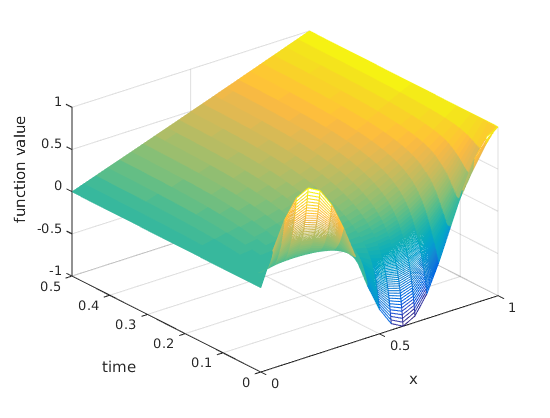
\includegraphics[scale = 0.45]{images/EulerHeat05.png}
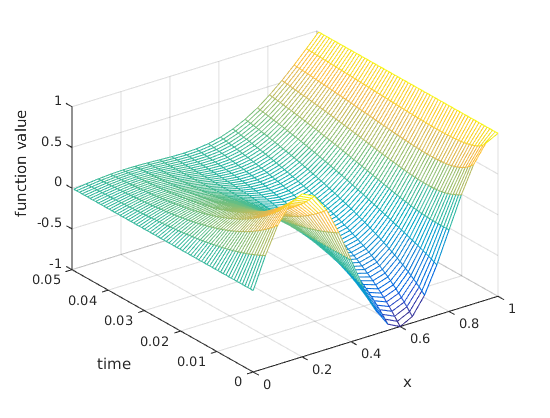
\includegraphics[scale = 0.45]{images/EulerHeat005.png}
\caption{Solution of the heat equation with the explicid Euler method. Until time $t = 0.5$ (left) and until $t = 0.05$ (right). The boundary conditions are: $0$, $1$, $sin(5\pi x/2)$.}
\label{fig:heatEulerStable}
\end{figure}
Running this code leads to the images in figure~\ref{fig:heatEulerStable}. The computations are done using a mesh ratio $\mu = 0.3$ and $\triangle x = \frac{1}{20}$. Therefore we have time steps of size $\triangle t = 0.00075 = 7.5 * 10^{-4}$. This scheme is stable for mesh ratios $\mu \leq 0.5$. Therefore if we increase the time step to $\approx 0.0013$ we are expecting to see instability. 
\begin{figure}
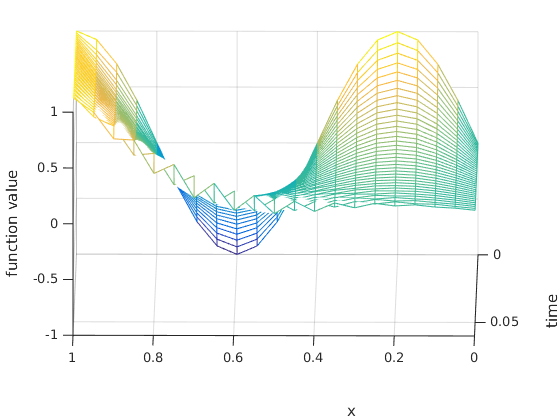
\includegraphics[scale = 0.6]{images/muUnstable.png}
\caption{Instabilities forming with $\mu = 0.55$ at time $t = 0.05$.}
\label{fig:heatEulerUnstable}
\end{figure}
A plot of forming instabilities is given in figure~\ref{fig:heatEulerUnstable}

\section{A slight variation of the problem}
Next we are going to consider a small variation of the problem. In fact the boundary conditions are going to change to:
\begin{equation*}
\phi(0,t) = 0, \; \phi(1,t) = 0, \; \phi(x,0) = sin(\pi x).
\end{equation*} 
For this set of boundary conditions we know the exact solution:
\begin{equation}
\pi(x,t) = exp(-\pi^2 t)sin(\pi x).
\end{equation}
Knowledge of the exact solution enables us to check the code we provided earlier. We are now able to compute the error in every grid point.
\begin{figure}
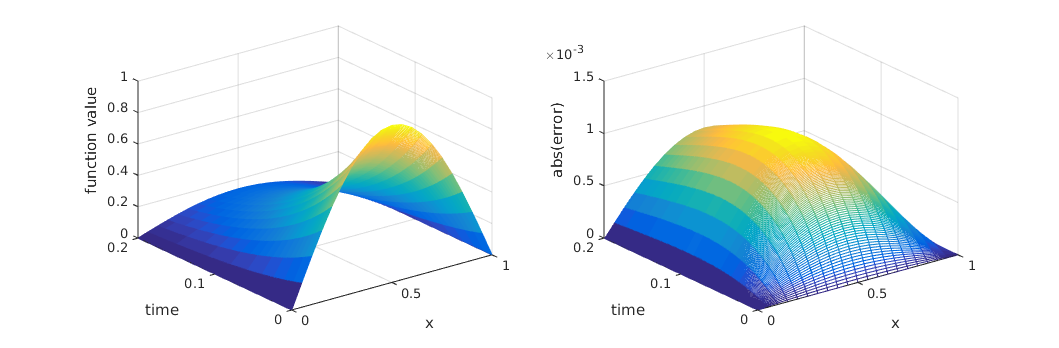
\includegraphics[scale = 0.45]{images/explicitEulerError.png}
\caption{Numerical solution of the heat equation with the second boundary value set (left). Absolute value of the numerical solution (right).}
\label{fig:errorExpEuler}
\end{figure}
 The solution should not deviate too much from the exact solution.\marginpar{TODO: more math here...} A plot of the numerical solution and it's error is given in figure~\ref{fig:errorExpEuler}. As the biggest error in any grid point is equal to $0.0011$ we conclude our implementation is probably correct.
  
\section{Euler, Crank-Nicolson and the $\theta$-method}
In this section we are going to use the more general theta-method-scheme to compare the errors of the explicit-Euler, implicit-Euler and Crank-Nicolson methods. $\Theta$-type methods are defined as \marginpar{$\partial_x^2$ denotes double application of a central difference}:
\begin{equation}
U_j^{n+1} - U_j^n = \mu [\theta \partial_x^2 U_j^{n+1} + (1-\theta) \partial_x^2 U_j^n].
\label{eq:theta}
\end{equation}
With $\theta = 0$ this we have the explicit Euler method, $\theta = 1$ leads to the implicit Euler method and finally $\theta = 0.5$ leads to the Crank-Nicolson method. In order do be able to implement a function in matlab that takes care of finding the error for each of these methods we have to derive two essential matrices. This is done by expanding the central differences from equation~\ref{eq:theta} and rearranging:
\begin{equation*}
-\mu \theta U_{j-1}^{n+1} + U_j^{n+1} ( 1 + 2\mu \theta) - \mu \theta U_{j+1}^{n+1}
\end{equation*}
\begin{equation}
= \mu (1 - \theta) U_{j-1}^n + (1 - 2\mu(1-\theta) U_j^n + \mu (1 - \theta) U_{j+1}^n.
\end{equation}
Here we are looking at an equation of the form $A \mathbf{U^{n+1}} = B \mathbf{U^{n}}$. Therefor the matrices $A$ and $B$ must be:
\begin{equation*}
A = \begin{pmatrix} 
(1 + 2\mu\theta) & -\mu\theta 	&		&		\\
-\mu\theta    & (1 + 2\mu\theta)& -\mu\theta	&		\\
	      &	 -\mu\theta	& (1+2\mu\theta)& -\mu\theta	\\
	      & \;\;\ddots	& \;\;\ddots	& \;\;\ddots	\\
		
\end{pmatrix}
\end{equation*}
\begin{equation}
B = \begin{pmatrix} 
1 - 2\mu(1-\theta) & \mu(1-\theta) 	&		&		\\
\mu(1-\theta)  	   & 1 - 2\mu(1-\theta)& \mu(1-\theta)&		\\
	      	    &	 \mu(1-\theta)	& 1 - 2\mu(1-\theta)& \mu(1-\theta)\\
	      	    & \ddots		& \ddots	& \ddots	\\
		
\end{pmatrix}.
\end{equation}
Now we are able to write the following function, which when executed with different thetas $\theta$ and grid parameters $\triangle x, \triangle t$ will allow us to learn more about the error. 
\lstinputlisting[language=matlab,caption={generic theta Method},label=lst:theta,captionpos=b]{code/theta.tex}
In the following section we will describe and interpret the results we obtained.

\subsection{Results}
\begin{table}
\begin{tabular}{|c|c|c|c|c|c|} \hline
			  & $\triangle x$ =1/20&$\triangle x$ =1/40&$\triangle x$ =1/80&$\triangle x$ =1/160&$\triangle x$ =1/320 \\ \hline 
$\triangle t$ =1/10	  & 0.8919 &   0.6577 &   0.4729 &   0.3368 &   0.2390	\\ 
$\triangle t$ =1/20	  & 0.1427 &   0.1119 &   0.0817 &   0.0584 &   0.0415	\\
$\triangle t$ =1/40	  & 0.0196 &   0.0214 &   0.0166 &   0.0121 &   0.0086	\\
$\triangle t$ =1/80 	  & 0.0047 &   0.0032 &   0.0035 &   0.0027 &   0.0019	\\ \hline
\end{tabular}
\caption{Error values of the Crank-Nicolson-scheme for different grid values. \textbf{Every entry has to be multiplied by 1.0e-03}.}
\label{tab:CN}
\end{table}
\begin{table}
\begin{tabular}{|c|c|c|c|c|c|} \hline
	& $\triangle x$ =1/20&$\triangle x$ =1/40&$\triangle x$ =1/80&$\triangle x$ =1/160&$\triangle x$ =1/320 \\
$\triangle t$ =1/10	& 0.0068  &  0.0049  &  0.0035  &  0.0025  &  0.0018 \\
$\triangle t$ =1/20	& 0.0023  &  0.0017  &  0.0012  &  0.0008  &  0.0006 \\
$\triangle t$ =1/40	& 0.0009  &  0.0007  &  0.0005  &  0.0003  &  0.0002 \\
$\triangle t$ =1/80	& 0.0004  &  0.0003  &  0.0002  &  0.0001  &  0.0001 \\ \hline
\end{tabular}
\caption{Error of the implicit Euler-scheme for different grid values.}
\label{tab:IE}
\end{table}
We proceeded to do a little more simulations where we took a little more space variables to look at the behaviour of the error in this direction. We choose to include two grid distances: $\Delta t = \frac{1}{10},\frac{1}{20}$. We then used 11 different grid spacings starting from $\frac{1}{40}$ and increasing by multiplying by 2. This was done for the crank-nicholson scheme and the implicit Euler. Results are shown in figure \ref{errorDX}.



We expect the error the behave like the consistency error for the general $\theta$-scheme. This is given by

\begin{eqnarray}
T^{n+1/2}_j = \left[{  (\frac{1}{2} - \theta) \Delta t u_{xxt} - \frac{1}{12}(\Delta x)^2 u_{xxxx}  }\right] + \left[{ \frac{1}{24} (\Delta t)^2u_{ttt} - \frac{1}{8}(\Delta t)^2u_{xxtt} }\right]  \\ + \left[{  \frac{1}{12} (\frac{1}{2}-\theta)   \Delta t (\Delta x)^2 u_{xxxxt} - \frac{2}{6!}(\Delta x)^4u_{xxxxxx}  }\right]
\label{Trunc}
\end{eqnarray}


So for the Crank Nicholson scheme where $\theta = 0$ we can easily find from \ref{Trunc} that $(T_j^{n+1/2})_{CN} = \mathcal{O}(\Delta(x)^2 + \Delta(t^2))$. Since we have held the time step constant in each experiment however, this means that as $\Delta x \rightarrow 0$ the error will bump into a constant term arising from the remaining finite time step size. We thus expect to see the quadratic behaviour as a constant slope in the part of the figure where $\Delta x$ is large enough in comparison to $\Delta t$ and more constant behaviour when $\Delta x$ is really small. In figure \ref{errorDX} we only see the constant slope, so we assume that the error arising from the time step size is still to small to notice.
For the implicit Euler we expect to have the same order in terms of $\Delta x$ but there is a difference in the time step dependent term.  $(T_j^{n+1/2})_{IE} = \mathcal{O}(\Delta(x)^2 + \Delta(t))$. We will not notice this in the general behaviour in this plot, because only space step size is plotted, which should have the same slope and this is what we see. We also notice that the error is generally larger than the Crank Nicholson scheme which could be attributed to the poor time step size dependency. 
\begin{figure}
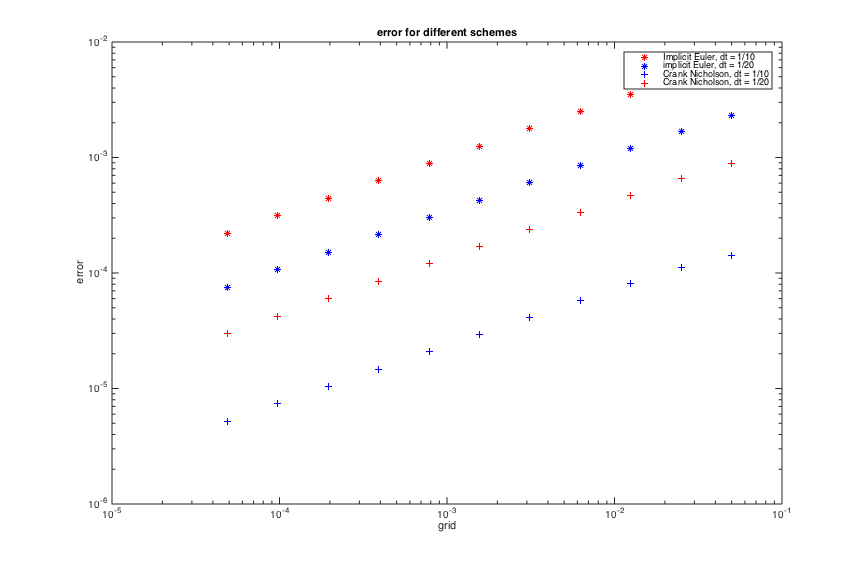
\includegraphics[scale = 0.45]{images/errorDX}
\caption{Plots show the behaviour of the error with grid spacing for Implicit euler and Crank Nicholson}
\label{errorDX}
\end{figure}

We have then repeated the experiment but instead let time step size vary. We used time steps starting from $\frac{1}{10}$ where every next one was half the size of the previous until we had 14 step sizes. We used these parameters for different grid sizes using again the Crank-Nicholson and the Implicit Euler. What do we expect to see? For Cranck Nicholson we had $(T_j^{n+1/2})_{CN} = \mathcal{O}(\Delta(x)^2 + \Delta(t^2))$. Which again means we expect to see a constant slope corresponding to the $(\Delta t)^2$ there where the time step sizes are large enough until we bump into the contant term arising from the constant grid size where grid spacing is so small its error is negatable in comparison. For Implicit Euler we have $(T_j^{n+1/2})_{IE} = \mathcal{O}(\Delta(x)^2 + \Delta(t))$. which is only first order in $\Delta t$ so we expect that this slope will be lower then the slope from crank nicholson. We can see all of this behaviour in figure \ref{errorDT}. 

\begin{figure}
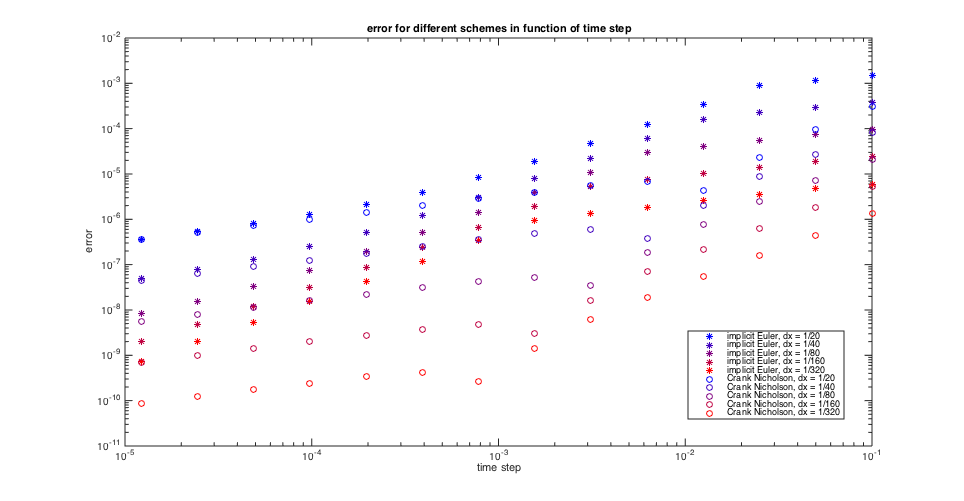
\includegraphics[scale = 0.45]{images/errorDT}
\caption{Plots show the behaviour of the error with time step spacing for Implicit euler and Crank Nicholson}
\label{errorDT}
\end{figure}

Note that it would also be interesting to include a similar plot using a constant $\mu$ instead of contant $\Delta t$ or $\Delta x$ for than we would not have to care about bumping in constant terms which would mean cleaner slopes. We could then more easily include explicit euler as we could just give it a sufficient $\mu$. But this has already been done and explained in the book corresponding to the course, so that would be uninteresting work.
    
      

%\begin{figure}
%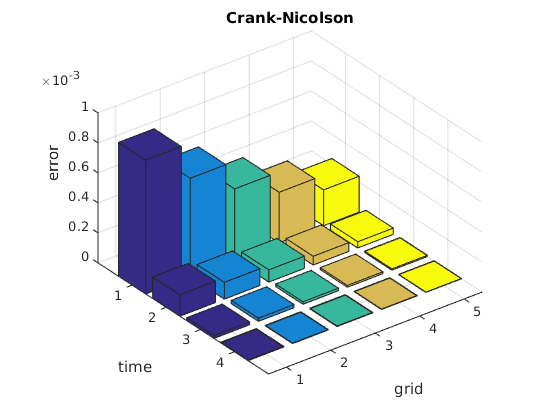
\includegraphics[scale = 0.45]{images/q2CN.png}
%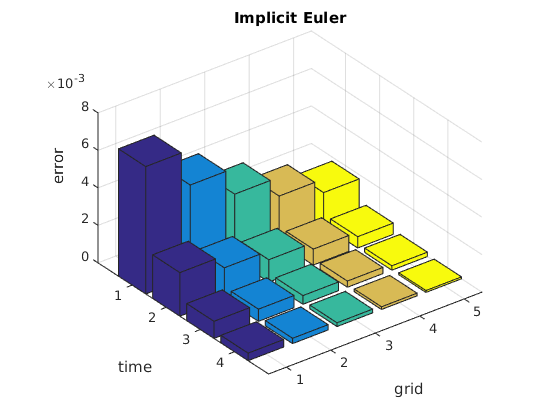
\includegraphics[scale = 0.45]{images/q2IE.png}
%\caption{Bar plots of the results shown in table~\ref{tab:CN} (left) and~\ref{tab:IE} (right).}
%\label{fig:bar}
%\end{figure}

\chapter{Heat Equation with convection}
In this part a convection term in introduced into the equation. We are now solving a different problem of the form:
\begin{equation}
\frac{\partial \phi}{\partial t} = a\frac{\partial \phi}{\partial x} + \frac{\partial^2 \phi}{\partial x^2}
\end{equation}
To solve this new problem we are forced to approximate the first derivative. We have three choices for these approximations central, forward and backward differences. The central difference approximates the derivative as:
\begin{equation}
a\frac{\partial \phi}{\partial x} \approx \frac{a_j^{n+1}}{2\triangle x}(U_{j+1}^{n+1} - U_{j-1}^{n+1})
\end{equation}
The forward difference approximation uses:
\begin{equation}
a\frac{\partial \phi}{\partial x} \approx \frac{a_j^{n+1}}{2\triangle x}(U_{j+1}^{n+1} - U_{j}^{n+1})
\end{equation}
And finally the backward difference approximation:
\begin{equation}
a\frac{\partial \phi}{\partial x} \approx \frac{a_j^{n+1}}{2\triangle x}(U_{j}^{n+1} - U_{j-1}^{n+1})
\end{equation} 
These approximations allow us to solve the problem. Results are shown in figure~\ref{fig:approx}.
\begin{figure}
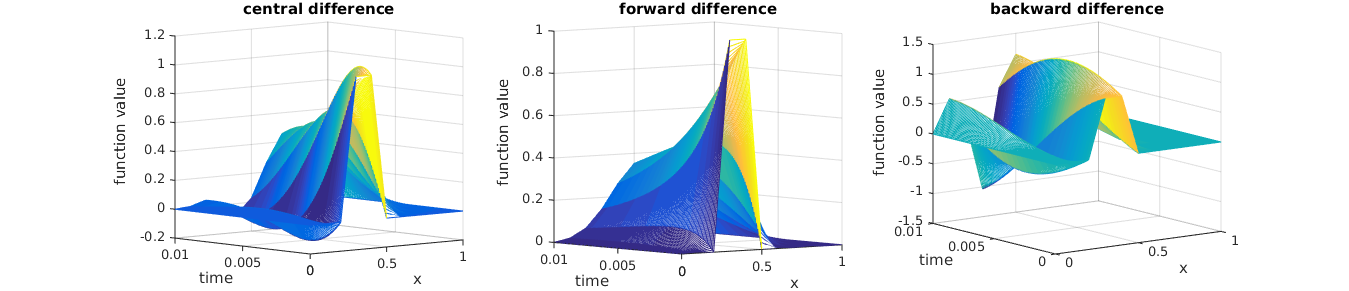
\includegraphics[scale = 0.4]{images/convection.png}
\caption{Solution of the problem with convection-term using different approximations for the first derivative term.}
\label{fig:approx}
\end{figure}
To do the computations we used $\triangle t = 0.0001$ and $\triangle x = 0.1$ which leads to $\mu = 0.01$.



\end{document}
